\documentclass{beamer}
\setbeamertemplate{navigation symbols}{}

\usepackage[polish]{babel}
\usepackage[utf8]{inputenc}
\usepackage{polski}
\usepackage[T1]{fontenc}
\usepackage{hyperref}

\usepackage{amsmath}
\usepackage{amsfonts}
\usepackage{amssymb}
\usepackage{amsthm}

\usetheme{Darmstadt}

\beamersetuncovermixins{\opaqueness<1>{25}}{\opaqueness<2->{15}}
\begin{document}
\title{Interfejs graficzny do układu\\ pozyskiwania modelu 3D \\ Projekt z przedmiotu SWIZ}  
\author{Piotr Róż \\ Jacek Zawistowski}
\institute
{
  Politechnika Warszawska\\
  Wydział Elektroniki i Technik Informacyjnych\\
}
\date{\today} 

\begin{frame}
\titlepage
\end{frame}

\section{Wstęp}
\begin{frame}\frametitle{Cel pracy}

  \begin{columns}
  
    \begin{column}{6cm}
      \begin{block}{Główna funkcjonalność}
	\begin{itemize}
	\item Utworzenie interfejsu do zestawu:
	  \begin{itemize}
	  \item projektor;
	  \item kamera. 
	  \end{itemize}\pause
	\item Oświetlenie analizowanego obiektu sekwencją obrazów.\pause
	\item Pobranie sekwencji obrazów z kamery.
	\end{itemize}
      \end{block}
    \end{column}
  
    \begin{column}{6cm}
      \begin{figure}[htb]
	\begin{center}
	  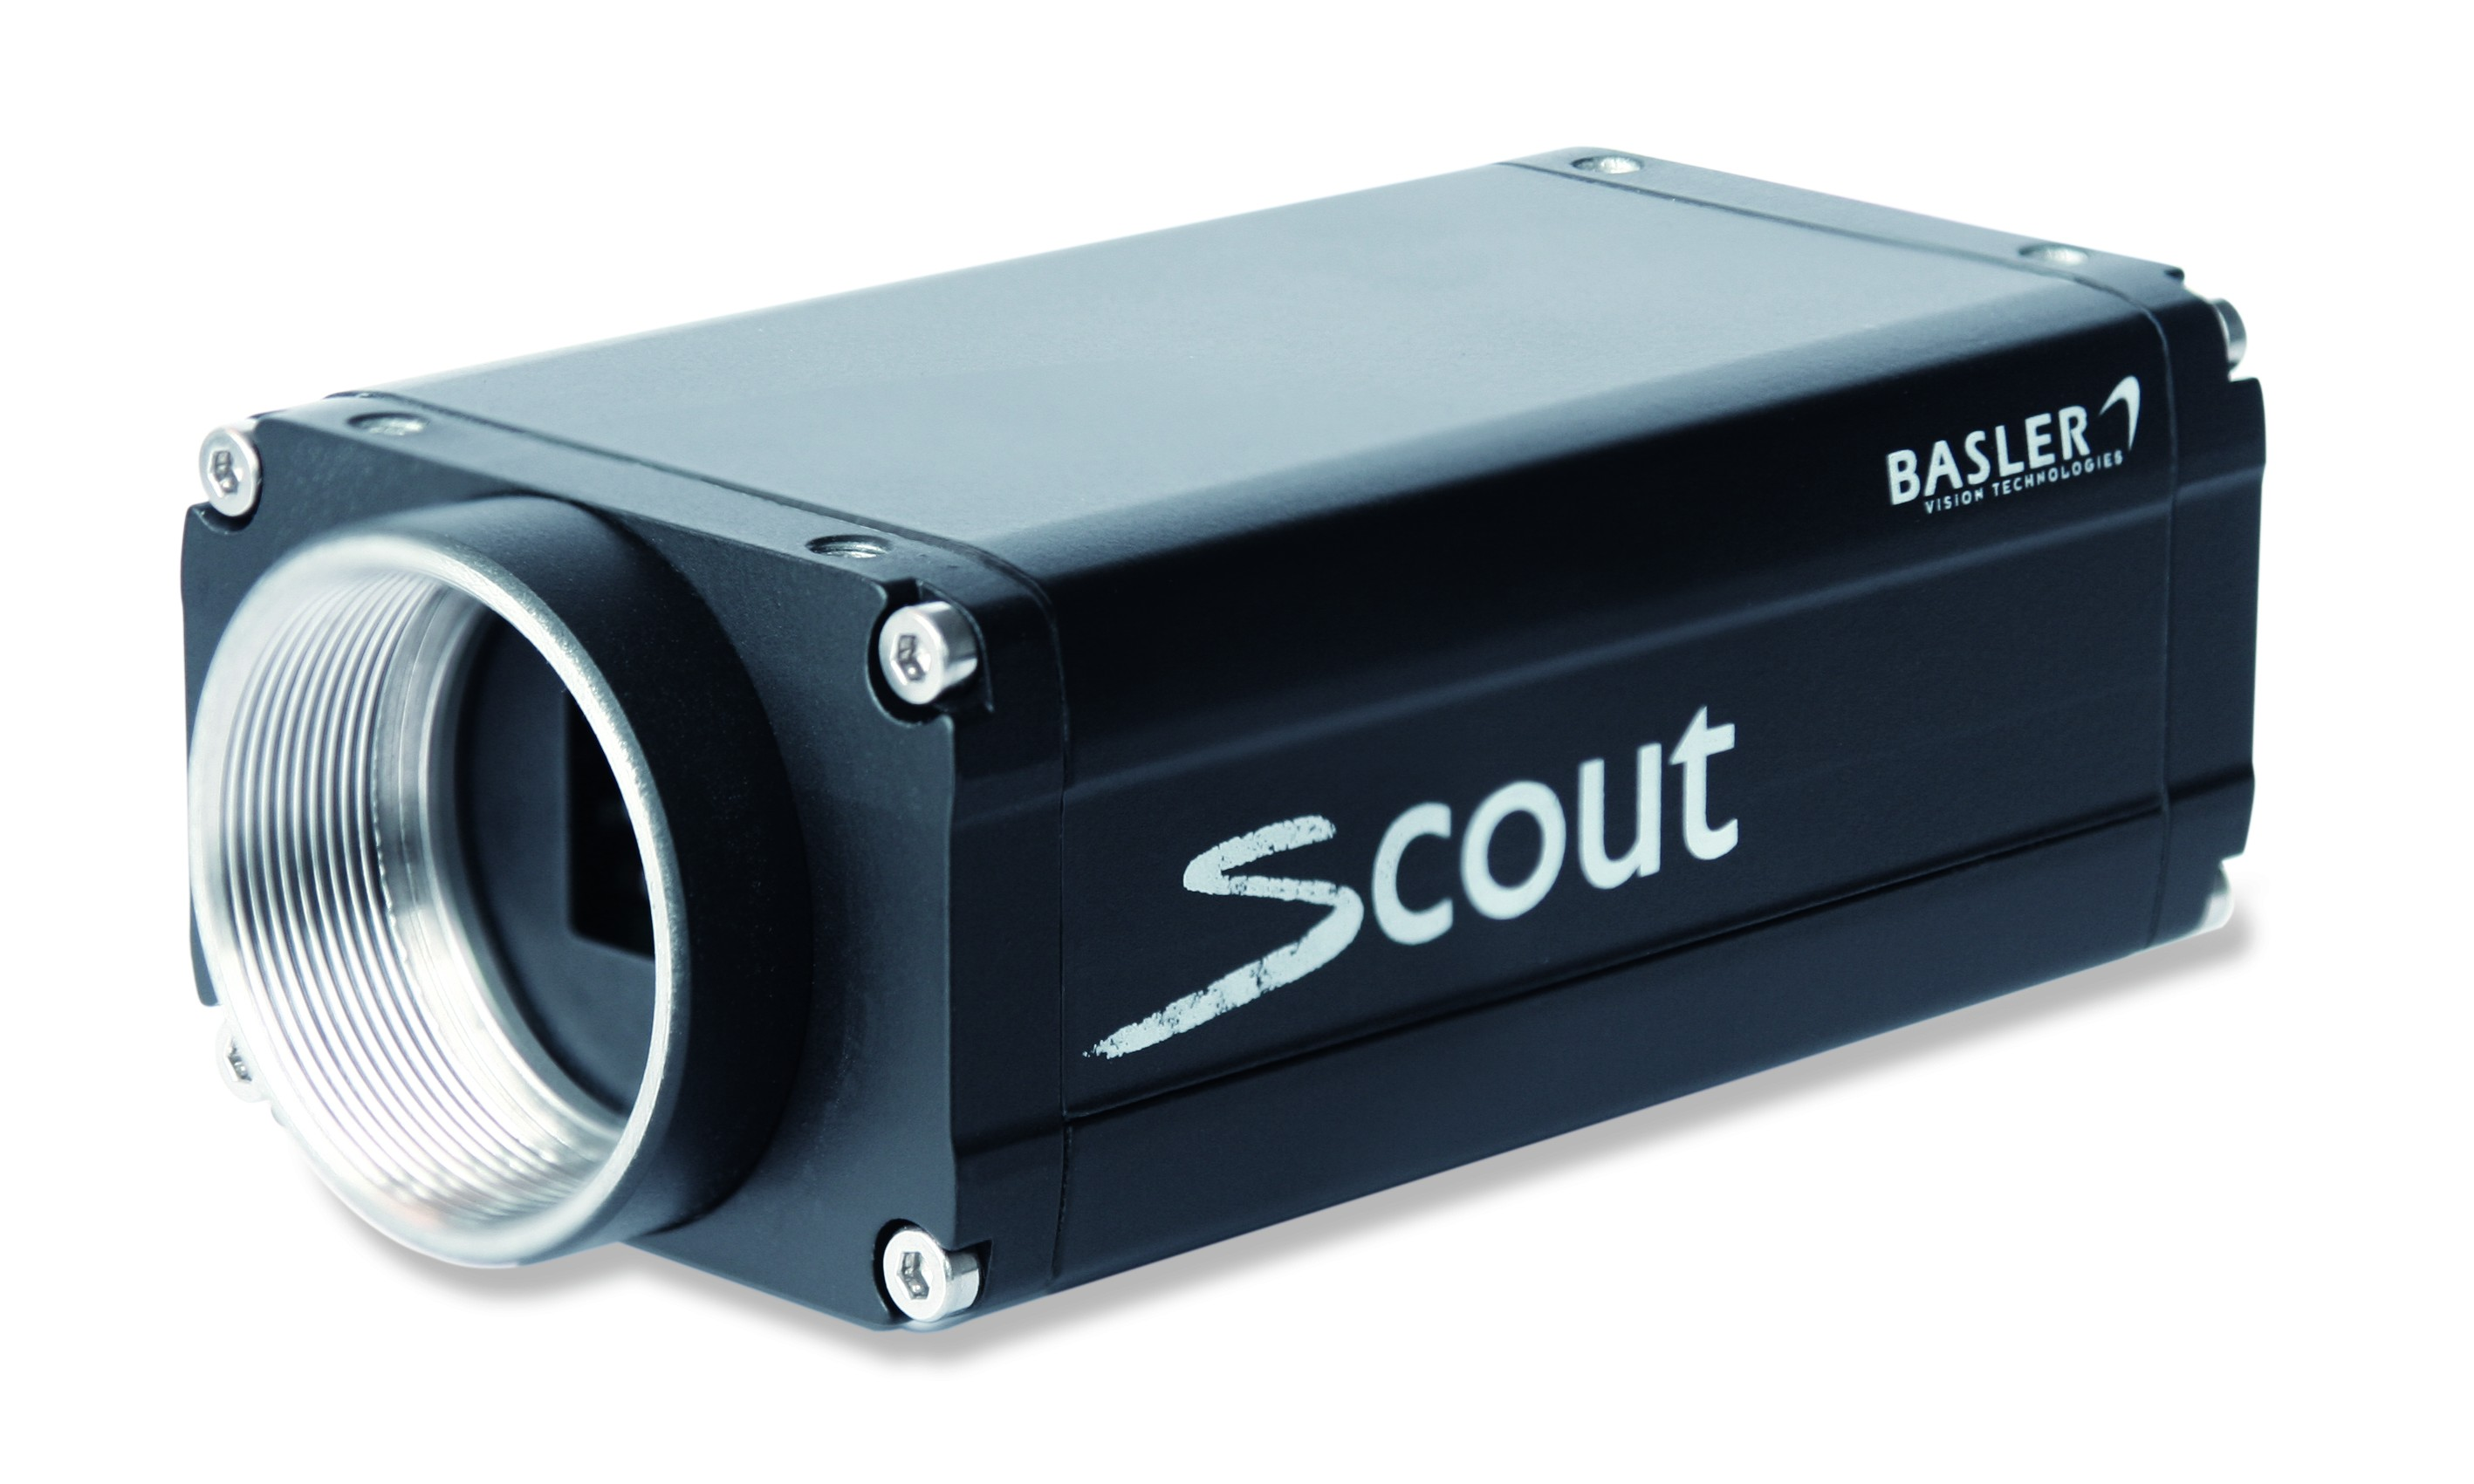
\includegraphics[angle=0,scale=0.05]{kamera.jpg}
	\end{center}
      \end{figure}
      
      \begin{figure}[htb]
	\begin{center}
	  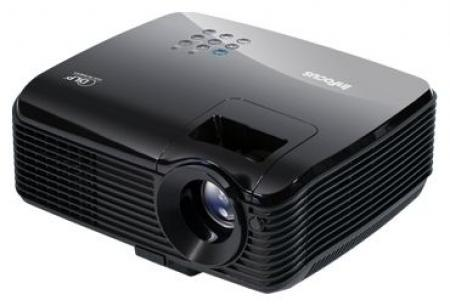
\includegraphics[angle=0,scale=0.2]{projektor.jpg}
	\end{center}
      \end{figure}
    \end{column}
    
  \end{columns}
  
\end{frame}


\begin{frame}\frametitle{Cel pracy}
  \begin{block}{Dodatkowa funkcjonalność}
    \begin{itemize}
    \item Implementacja podstawowych operacji matematycznych na obrazach:
      \begin{itemize}
      \item dodawanie;
      \item odejmowanie;
      \item mnożenie;
      \item itd
      \end{itemize}
	kolejnych \textbf{n} obrazów.\pause
    \item Tworzenie wizualizacji 3D pobranych obrazów.\pause
    \item Implementacja dodatkowych algorytmów w celu analizy pozyskanej sekwencji obrazów.
    \end{itemize}
  \end{block}
\end{frame}


\section{Architektura}
\subsection{Architektura systemu}
\begin{frame}\frametitle{Sekwencja działań}
      \begin{enumerate}
       \item Użytkownik wybiera predefiniowane obrazy do wyświetlenia na analizowanym obiekcie.\pause
       \item Wybrane obrazy tworzą sekwencję, która oświetla obiekt.\pause
       \item Użytkownik ustala parametry wyświetlanej sekwencji: 
       \begin{itemize}
        \item czas wyświetlania jednego obrazu;
        \item odstęp między kolejnymi obrazami;
        \item itd.
       \end{itemize} \pause
       \item Wyświetlana sekwencja zapisywana jest do pliku wideo.\pause
       \item Obraz pozyskiwany z kamery jest wyświetlany w czasie rzeczywistym oraz zapisywany do pliku wideo.
      \end{enumerate}
\end{frame}

\subsection{Architektura oprogramowania}
\begin{frame}\frametitle{Schemat}
  
    \begin{columns}
    
      \begin{column}{6cm}

	\begin{itemize}
	\item Akwizycja obrazu za pomocą biblioteki OpenCV, poprzez interfejs Ethernet, bezpośrednie połączenie przez framegrabber lub usb.\pause
	\item Wyświetlanie obrazu w trybie pełnoekranowym poprzez złącze wideo D-Sub/DVI/HDMI.\pause
	\item Wykorzystane biblioteki: 
	  \begin{itemize}
	    \item OpenCV;
	    \item PCL;
	    \item Qt;
	    \item ewentualnie OpenGL.
	  \end{itemize}
	\end{itemize}
	
      
      \end{column}
    
    \begin{column}{6cm}
     
      \begin{figure}[htb]
	\begin{center}
	  
\includegraphics[angle=0,scale=0.3]{opencv.png}
	\end{center}
      \end{figure}
      
      \begin{figure}[htb]
	\begin{center}
	  
\includegraphics[angle=0,scale=0.05]{pcl.png}
	\end{center}
      \end{figure}
      
      \begin{figure}[htb]
	\begin{center}
	  
\includegraphics[angle=0,scale=0.15]{qt.png}
	\end{center}
      \end{figure}
      
      \begin{figure}[htb]
	\begin{center}
	  
\includegraphics[angle=0,scale=0.2]{opengl.jpg}
	\end{center}
      \end{figure}
     
    \end{column}

  \end{columns}
    
\end{frame}

\section{Podsumowanie}
\begin{frame}\frametitle{Podsumowanie}

  \begin{block}{Zalety}
   \begin{itemize}
    \item Wieloplatformowość aplikacji.
    \item Przenośność bibliotek.
    \item Możliwość wyboru między różnymi językami programowania: C++, Python...
   \end{itemize}

  \end{block}


  \begin{alertblock}{Możliwe problemy}
    \begin{itemize}
     \item Synchronizacja obrazów z projektora i kamery.
     \item ?
    \end{itemize}
  \end{alertblock}
\end{frame}

\begin{frame}\frametitle{Dziękujemy}
\begin{center}
  \Huge{\textbf{Dziękujemy za uwagę!}}
\end{center}
\end{frame}

\end{document}